\begin{frame}
 \frametitle{Applications of Cross Product}

\only<1>{Vector perpendicular to given vectors $\textbf{u}$ and $\textbf{v}$: $\textbf{u} \times \textbf{v}$.\\
Example: Vector perpendicular to $\textbf{u} = \textbf{i}+\textbf{j}$ and $\textbf{v}=\textbf{j}+\textbf{k}$:
%
\begin{align*}
 \textbf{w} = & (\textbf{i}+\textbf{j}) \times (\textbf{j}+\textbf{k}) =
\textbf{i} \times \textbf{j} + \textbf{i} \times \textbf{k} +
\textbf{j} \times \textbf{j} + \textbf{j} \times \textbf{k} = \\
 = & \textbf{k} -\textbf{j}+\textbf{0}+\textbf{i} = \textbf{i} - \textbf{j} + \textbf{k}\; .
\end{align*}}

\only<2->{$A$, $B$, $C$ points in space, $\textbf{u} = \textbf{AB}$, $\textbf{v}=\textbf{AC}$. Then \\
%
\begin{figure}[h]
  \psfrag{u}{$\textbf{v}$}
  \psfrag{v}{$\textbf{u}$}
  \psfrag{w}{$\textbf{w}$}
    \psfrag{A}{$A$}
    \psfrag{B}{$B$}
    \psfrag{C}{$C$}
    \psfrag{D}{$D$}
  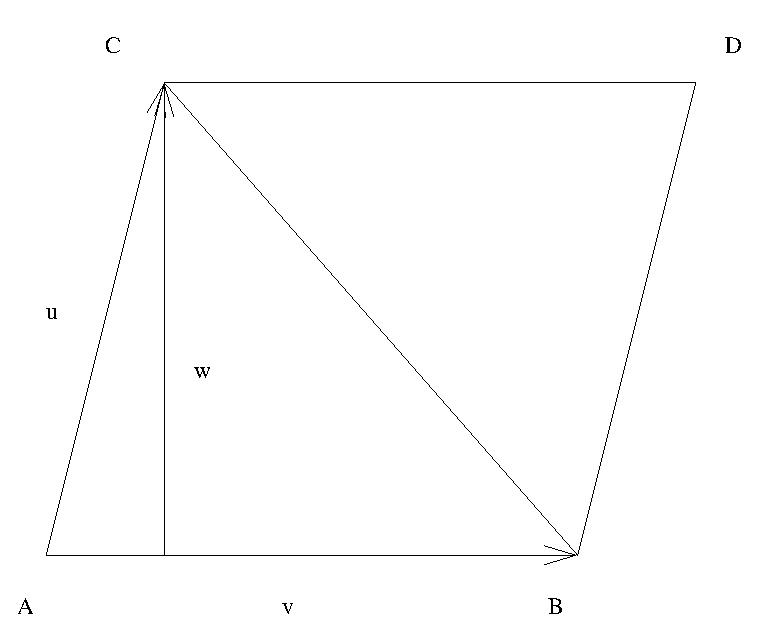
\includegraphics[height=1in]{../../modules/vectors/pictures/ok-area_triangle.eps}
\end{figure}
%
$$|\textbf{w}| = |\textbf{orth}_{\bm{u}} \textbf{v}| = \text{ distance from } C \text{ to } AB\; .$$
%
$$|\textbf{u} \times \textbf{v}| = |\textbf{orth}_{\bm{u}} \textbf{v}| \, |\textbf{u}| =
2 \text{area}(ABC) = \text{area}(ABDC)$$
%
$|\textbf{u} \times \textbf{v}|$ = Area of parallelogram on sides $\textbf{u}$ and $\textbf{v}$.
\pause

Example: Area of triangle $A(1,2,3)$, $B(2,3,1)$, $C(3,1,2)$
%
$$\text{Area}(ABC) = \frac{1}{2}|\textbf{AB} \times \textbf{AC}| =
\frac{1}{2}|\langle 1,1,-2\rangle \times \langle 2, -1, -1\rangle | = $$
%
$$= \frac{1}{2} |\langle -3, -3, -3 \rangle| = \frac{3\sqrt{3}}{2}\; .$$}

\end{frame}